\subsection{Mathematical Primer: Basic Models}

A review of some basic and advanced statistical methodologies that are useful for developing trading strategies.

\subsubsection{Univariate Time Series Models}

Trading activities through an exchange can be described by a sequence of time stamps ('ticks') $t_0 < t_1 < \cdots < t_n$, and 'marks' $y_i$ at time $t_i$, where $t_i$ denote market open, $t_n$ denote market close. The marks $y_i$ is a characteristic of the order book at time of $i$th activity. Events with marks associated with the ticks can be described mathematically as a marked point process.
\begin{figure}[H]
\centering
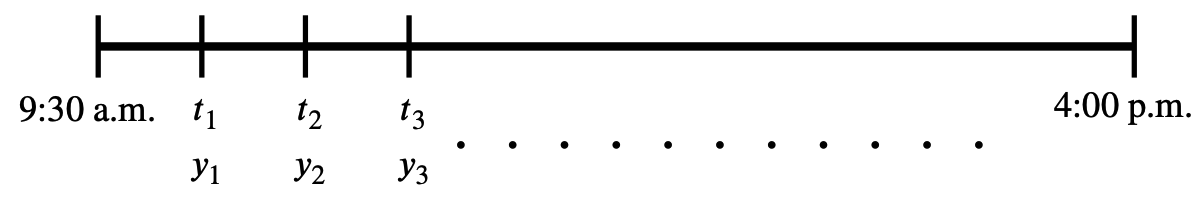
\includegraphics[scale=0.4]{/fundamentals/ticksandmarks}
\caption{Ticks and Marks}
\end{figure}

A data aggregation method is where aggregation is conducted when there is a change in marker. An alternative aggregation method would be to divide the time span $T$ for exchange hours into $K$ intervals, so regularly spaced intervals are of size $\Delta t = T/K$. The time series method to be discussed will apply to all aggregated data.\\

Let $p_{it} = \ln P_{it}$ denote price of $i$th asset at time $t$; $p_t = (p_{1t}, p_{2t}, \ldots, p_{nt})$ denote price vector for $n$ assets; $y_{it}$ denote vector of characteristics of $i$th asset at time $t$. These quantities are aggregated from high frequency data. Consider $r$ factors $f_t = (f_{1t}, f_{2t}, \ldots, f_{rt})$ that may include market and industry factors, and asset characteristics. Trading rules can be broadly grouped as follows:
\begin{enumerate}[label=\roman*.]
\setlength{\itemsep}{0pt}
\item \hlt{Statistical Arbitrage}: $E(p_{i, t+1} \ \vert \ p_{i,t}, p_{i, t-1}, \ldots, y_{i,t}, y_{i, t-1}, \ldots)$, that predicts the price of $i$th stock at $t+1$ based on past trading information (also known as time series momentum)
\item \hlt{Momentum}: $E(p_{t+1} \ \vert \ p_t, p_{t-1}, \ldots, y_t, y_{t-1}, \ldots)$, that predicts the cross-sectional momentum of a subset of stocks based on past trading characteristics. For portfolio formation and rebalancing, pairs trading
\item \hlt{Fair Value}: $E(p_{t+1} \ \vert \ p_{t}, p_{t-1}, \ldots, y_t, y_{t-1}, \ldots, f_t, f_{t-1}, \ldots)$, predicts price using all relevant quantities. Factors normally include market, Fama-French; at a more macro level than timescale considered for price prediction, but may still be useful.
\end{enumerate}

Hence price and volatility prediction can be formulated as a tie series prediction problem. Autocorrelations and partial autocorrelations can be used to build autoregressive and ARCH models with some predictive power.


